\section{Informed search}
\graphicspath{{images/}}
% ============================================= A*  ============================================= 
\subsection{Question 4 - A* search  algorithm}
% enuntul intrebarii
In sectiunea urmatoare va fi descris exercitiul 3.2 din laborator \newline


\textit{"Go to aStarSearch in search.py and implement \textbf{A* search algorithm}. A* is graphs search with the frontier as a priorityQueue, where the priority is given bythe function g=f+h"}.


\subsubsection{Code implementation}
In continuare se regaseste codul propus pentru implemetarea acestui algoritm de cuatare. In incercarea de implementare si apoi testare a solutiei propuse s-au apelat mai multe comenzi din terminal pentru a vedea evolutia agentului pacman in procesul de cautare a solutiei sale \\

\textbf{Code:}
% a se completa fisierul code/4_a_star.py
\begin{listing}[h]
    \inputminted[linenos]{python}{code/04_a_star.py}
    \caption{Solution for the A* algorithm.}
    \label{listing:a_star}
\end{listing}


\textbf{Explanation:}
\begin{itemize}
    \setlength\itemsep{0em}
    \item in cadrul acestui algoritm este nevoie de o structura de date speciala pentru frontiera. Aceasta structura va fi PriorityQueue, iar prioritatea nodurilor ce se vor afla in frontiera va fi data de costul drumului pana in acel nod si de estimarea costului pana la scop(determinata prin intermediul unei euristici). La linia 11 este creata o astfel de structura pe care o gasim implementata in util
    \item pentru nod-uri s-a folosit aceeasi structura folosita si in cadrul solutiei pentru dfs si bfs
    \item ideea acestui algoritm este de a alege din frontiera nodul cel mai bun ca si candidat pentru solutia optima, nod ce va fi testat daca e scop si in caz afirmativ se va returna solutia sau in caz contrar ii vor expandati succesorii si adaugati in frontiera daca nu au fost expandati inainte. 
    \item linia 29 este esentiala in cadrul acestei solutii, deoarece daca pentru un nod se gaseste un copil ce se afla in frontiera, prioritatea acetuia se va modifica daca functia de evaluare a costului in aceasta conjuctura e mai mica decat cea de dinainte. Aceasta va determina intotdeuana o solutie optima a algoritmului. 
    \item pentru a construi calea de la nodul de start la nodul scop cu actiunile necesare se va apela functia \textbf{construct\_path(node)}

\end{itemize}


\textbf{Commands:}
\begin{itemize}
    \setlength\itemsep{0em}
    \item  -l bigMaze -z .5 -p SearchAgent -a fn=astar,heuristic=manhattanHeuristic
    \item  -l mediumMaze -z .5 -p SearchAgent -a fn=astar,heuristic=manhattanHeuristic
        
\end{itemize}

\subsubsection{Questions}
This sub-section is dedicated to the additional questions that come along with the exercise. Please answer to the following questions:\newline


\textbf{Q1:} Does A* and UCS find the same solution or they are different?


\textbf{A1:} Depinde de euristica folosita pentru estimarea costului pana la nodul scop. Daca euristica este constana 0, atunci A* star este identinc cu UCS, iar daca euristica e buna (admisibila si consistenta) A* ar trebui sa ofere aceeasi solutie ca UCS, solutie care e si optima de altfel.


\textbf{Q2:} Does A* finds the solution with fewer expanded nodes than UCS?


\textbf{A2:} Cu cat euristica se apropie de adevar, cu atat algoritmul va expanda mai putine noduri, deaorece el se va duce pe o abordare de tip Greedy. Deoarece A* are in logica sa si o abordare de tip Greedy, el va expanda mai putine noduri decat UCS.

\textbf{Q3:} Run autograder \textit{python autograder.py} and write the points for Question 4 (min 3 points).


\textbf{A3:} Question q3: 4/4


\subsubsection{Personal observations and notes}
Pentru bigMaze costul total al caii este de 210, iar numarul de noduri explorate este de 549.Pentru medium-Maze costul total al caii este de 68, iar numarul de noduri explorate este de 221.S-a folosit pentru aceste teste euritstica \textit{manhattan} Observam ca avem solutia optima pentru cele doua probleme, iar numarul de noduri expandate este mai putin decat la bfs.
\vspace{0.75cm}

% ============================================= All Corners ===================================== 
\subsection{Question 5 - Find all corners - problem implementation}
% enuntul intrebarii
In urmatoare subsectiune va fi prezentat exercitiul 3.3 din laborator al carui enunt e: \newline


\textit{"Pacman  needs  to  find  the  shortest  path  to  visit  all  the  corners,regardless  there  is  food  dot  there  or  not. Go to \textbf{CornersProblem} in searchAgents.py and propose a representation of the state of this search problem. It might help to look at the existing implementation for PositionSearchProblem. The representation should include only the information necessary to reach the goal. Read carefully the comments inside the class CornersProblem."}.


\subsubsection{Code implementation}
In continuare se regaseste codul propus pentru implemetarea acestei clase ce descrie o noua problema. In incercarea de implementare si apoi testare a solutiei propuse s-au apelat mai multe comenzi din terminal pentru a vedea evolutia agentului pacman in procesul de cautare a solutiei sale \\

\textbf{Code:}

% a se completa fisierul code/corner_problem.py
\inputminted[linenos]{python}{code/05_corner_problem.py}


\textbf{Explanation:}
\begin{itemize}
    \setlength\itemsep{0em}
    \item  la linia 24 este declarat un atribut al \textit{problemei} ce se refera la starea colturilor. Va fi declarat un dictionar de forma \textbf{colt:vizitat?}- unde prin \textit{vizitat?} se intelege o valoare buleana (True sau False). Acest dictionar va contine informatia despre toate colturile.
    \item la liniile 30 -32 se verifica pentru fiecare colt daca e pozitia de start sau in acel loc e un zid si in caz afirmativ il vom marca vzitat in dictionarul atribut
    \item la linia 37 se va lua o tupla pentru pozitia de start, care va contine pozitia in grid si dictionarul cu informatia despre colturi
    \item metoda \textbf{getStartState} va returna tupla formata din starea initiala si starea colturilor la momentul initial
    \item scopul problemei de fata este de a vizita toate colturile. Se ajunge la scop in momentul in care toate valorile din dictionar sunt true. Metoda \textbf{isGoalstate(self,state)} va fi implementata printr-o simpla parcurgere a valorilor din dictionar si daca se intalneste o valoare de False va returna False, iar daca nu, va returna True
    \item liniile 58-79: metoda \textbf{expand} este similara cu cea de la \textit{PositionSearchProblem} 
    \item liniile 105-122 ceea ce lipseste in metoda \textbf{getnextState} este determinarea noului dictionar al colturilor asociat starii.
\end{itemize}

\textbf{Commands:}
\begin{itemize}
    \setlength\itemsep{0em}
    \item  -l mediumCorners -p SearchAgent -a fn=bfs,prob=CornersProblem
    \item  -l mediumCorners -p SearchAgent -a fn=astar,heuristic=cornersHeuristic,prob=CornersProblem
    \item   -l mediumCorners -p SearchAgent -a fn=astar,prob=CornersProblem
\end{itemize}
\subsubsection{Questions}

\textbf{Q1:} For mediumCorners, BFS expands a big number - around 2000 search nodes.  It’s time to see that A* with an admissible heuristic is able to reduce this number. Please provide your results on this matter. (Number of searched nodes).

\textbf{A1:} Bfs: 1966 noduri expandate; O euristica admisibila pentru aceasta problema poate fi nullEuristic. Pentru aceasta euristica numarul de noduri expandate a ramas 1966. Pentru cazul in care am apelat cu o eurirstica consistenta si admisibila (cornersHeuristic -implementatata in sectiunea urmatoare), numarul s-a redus la 783 de noduri expandate.


\subsubsection{Personal observations and notes}
Initial am creat o clasa \textbf{CornerState} care imi descria structura pentru o stare din aceasta problema apoi am vazut ca se doreste folosirea unei tuple, deoarece cand se prelua pozitia se dorea indexarea (state[0] -linia 85) 
\vspace{0.75cm}

% ============================================= Consistent heuristic ============================= 
\subsection{Question 6 - Find all corners - Heuristic definition}
% enuntul intrebarii
In sectiunea aceasta este explicat si rezolvat exercitiul 3.4 din laborator:  \newline


\textit{"Implement  a  consistent  heuristic  for  CornersProblem. Go to the function \textbf{cornersHeuristic} in searchAgent.py."}.


\subsubsection{Code implementation}
 In continuare se regaseste codul propus pentru implemetarea acestei metode ce descrie o euristica consistenta pentru problema CornersProblem. In incercarea de implementare si apoi testare a solutiei propuse s-au apelat mai multe comenzi din terminal pentru a vedea evolutia agentului pacman in procesul de cautare a solutiei sale \newline\newline\\


\textbf{Code:}

% a se completa fisierul code/6_consisntency_heuristic.py
\inputminted[linenos]{python}{code/06_consistent_heuristic.py}


\textbf{Explanation:}
\begin{itemize}
    \setlength\itemsep{0em}
    \item pentru ca o euristica sa fie consistenta si admisibila ea trbuie sa indeplineasca niste conditii:\newline
    \textbf{admisibilitate}: h(n) <= h*(n) , unde h* este costul real pana la cel mai apropiat scop; in acest caz se va elimina supraestimarea costului \newline
    \textbf{consistenta}: se poate determina cu regula triunghiului; 
    \begin{itemize}
    \setlength\itemsep{0em}
    \item fie n si n' doua stari din spatiul starilor problemei. 
    \item h(n) - h(n') <= c(n,a,n');
    \item h(n)-costul estimat din n pana la scop, 
    \item h(n')- costul estimatdin n' , 
    \item iar c(n,a,n') - este costul real de tranzitie din starea n in n' prin actiunea a
    \end{itemize}
    
    \item o euristica consistenta e si admisibila
    \item euristica pe care am propus-o se descrie astfel: Se calculeaza distanta din punctul curent la coltul cel mai apropiat de el, iar apoi se calculeaza distanta de la acel colt la coltul cel mai indepartat de acel colt. Prin distanta ma refer la distanta manhattan. Euristica va fi suma dintre cele doua distante calculate
    \item \begin{figure}[htp]
         \centering
         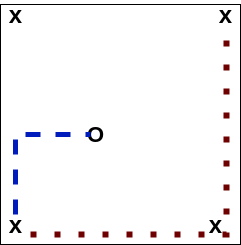
\includegraphics[width=4cm]{text/images/corner.png}
         \caption{O posibila stare initiala}
         \label{fig:corner}
         \end{figure}
    \item ideea consta in faptul ca daca agentul alege sa mearga la cel mai apropiat colt de el, va suporta consecinta de a merge din acel colt la cel mai indepartat colt de coltul respectiv 
    \item liniile 18-21: se extrag colturile nevizitate cand agentul e in starea \textit{state}
    \item liniile 23-24: se rezolva situatia in care starea e scop si atunci euristica trbeuie sa returneze valoarea 0
    \item linia 27: calculare distanta cea mai scurta catre un colt cu manhattan facandu-se abstractie de pereti
    \item linia 31: calculare distanta cea mai lunga catre un colt din coltul determinat la instructiunea precedenta 
    \item 34 : euristica va fi suma dintre aceste doua distante \newline
\end{itemize}


\textbf{Commands:}
\begin{itemize}
    \setlength\itemsep{0em}
    \item -l mediumCorners -p SearchAgent -a fn=aStarSearch,prob=CornersProblem,heuristic=cornersHeuristic
    \item  -l bigCorners -p SearchAgent -a fn=aStarSearch,prob=CornersProblem,heuristic=cornersHeuristic
\end{itemize}

\subsubsection{Questions}

\textbf{Q1:} Test  with  on the mediumMaze layout. What is your number of expanded nodes?

\textbf{A1:} 783 numarul total de noduri expandate, iar costul e de 106


\subsubsection{Personal observations and notes}
% descrieti aici orice fel de probleme ati intampinat in timpul rezolvarii acestui task si modul cum in care le-ati solutionat

% ============================================= Food heuristic ============================= 
\subsection{Question 7 - Eat all food dots - Heuristic definition}
% enuntul intrebarii
In urmatoarele paragrafe va fi prezentata rezolvarea exercitiului 3.5 dib laborator: \newline


\textit{"Propose a heuristic for the problem of eating all the food-dots. The problem of eating all food-dots is already implemented in \textbf{FoodSearchProblem} in searchAgents.py."}.


\subsubsection{Code implementation}
 In continuare se regaseste codul propus pentru implemetarea acestei metode ce descrie o euristica consistenta pentru problema CornersProblem. In incercarea de implementare si apoi testare a solutiei propuse s-au apelat mai multe comenzi din terminal pentru a vedea evolutia agentului pacman in procesul de cautare a solutiei sale \newline \\

\textbf{Code:}

% a se completa fisierul code/6_consisntency_heuristic.py
\inputminted[linenos]{python}{code/07_find_food.py}


\textbf{Explanation:}
\begin{itemize}
    \setlength\itemsep{0em}
    \item ideile prezentate in sectiunea anterioara sun valabile si pentru aceasta subsectiune
    \item ideea este asemnatoare cu cea de la cornerHeuristic
    \item la liniile 5-6: se rezolva cazul in care starea curenta e scop, caz in care euristica trebuie sa fie 0
    \item la linia 10: se calculeaza distanta de la agent pana la cea mai apropiata bucata de mancare, si se determina si pozitia acesteia
    \item la linia 11: se calculeaza distanta de la bucata de mancare determinata anterior pana la cea mai indepartata bucata de mancare fata de aceasta. 
    \item euristica va fi data de suma acestor doua distante
    \item ideea de la care am plecat a fost ca daca agentul alege calea cea mai usoara (adica se indreapta spre cea mai apropiata bucata de mancare), el va suporta consecinta de a merge de la acea bucata de mancare pana la cea mai indeparatata bucata de mancare
\end{itemize}


\textbf{Commands:}
\begin{itemize}
    \setlength\itemsep{0em}
    \item -l testSearch -p SearchAgent -a fn=astar,prob=FoodSearchProblem,heuristic=foodHeuristic
\end{itemize}

\subsubsection{Questions}

\textbf{Q1:} Test  with  autograder \textit{python autograder.py}. Your score depends on the number of expanded states by A* with your heuristic. What is that number?

\textbf{A1:} Numarul de noduri expandate: 8178





% ============================================= SUBOPTIMAL ============================================= 
\subsection{Question 8 - Suboptimal Search}
% enuntul intrebarii
In aceasta sectiune este prezentata o metoda suboptimala:\newline

\textit{"Implement the function findPathToClosestDot in searchAgents.py. Our agent solves this maze (suboptimally!) in under a second with a path cost of 350:"}


\subsubsection{Code implementation}
In continuare se regaseste codul propus pentru implemetarea clasei \textbf{AnyFoodSearchProblem} care decrie o problema ce se poate rezolva suboptimal. In incercarea de implementare si apoi testare a solutiei propuse s-au apelat mai multe comenzi din terminal pentru a vedea evolutia agentului pacman in procesul de cautare a solutiei sale \newline \\


\textbf{Code:}
% a se completa fisierul code/ucs.py
\inputminted[linenos]{python}{code/08_suboptimal.py}

\textbf{Explanation:}
\begin{itemize}
    \setlength\itemsep{0em}
    \item ideea consta in faptul ca agentul mananca de fiecare data cea mai apropiata bucata de mancare, ceea ce ii confera o logica greedy de rezolvare a solutiei
    \item in aceste conditii, metoda \textbf{isGoalState(self, state)} a problemei \textit{AnyFoodSearchProblem} este foarte simpla si se rezuma la verificarea daca starea curenta prezinta o pozitie cu mamncare sau nu. In cazul in care e pozitie cu mancare se va returna True.
    \item in metoda \textbf{findPathToClosestDot}, determinarea actiunilor se va face cu ajutorul parcurgerii bfs pe problema \textit{AnyFoodSearchProblem}, aceasta parcurgere radiala va duce la cea mai scurta cale spre scop

\end{itemize}


\textbf{Commands:}
\begin{itemize}
    \setlength\itemsep{0em}
    \item  -l bigSearch -p ClosestDotSearchAgent -z .5
        
\end{itemize}

\vspace{0.75cm}

\subsection{References}
R. Stuart, N. Peter, Artificial Intelligence: A Modern Approach, 4th US ed., capitol 3, [online] \newline
Curs Inteligenta Artficiala, Universitatea Tehnica din Cluj Napoca, furnizat: moodle.cs.utcluj.ro